\sect{Lineare Abbildungen}

\ssect{Definition}

Seien $V$ und $W$ zwei reelle Vektorräume und $f: V \rightarrow W$ eine Abbildung des Vektorraums $V$ in den Vektorraum $W$.
Die Abbildung $f$ ist eine \textbf{lineare Abbildung}, falls $\forall \vec{x}_1, \vec{x}_2 \in V$ und $\forall \lambda \in \R$ gilt:
\begin{itemize}
    \item $f(\vec{x}_1 + \vec{x}_2) = f(\vec{x}_1) + f(\vec{x}_2)$
    \item $f(\lambda \vec{x}_1) = \lambda f(\vec{x}_1)$
\end{itemize}

\textbf{Satz:} Für jede lineare Abbildung $f: V \rightarrow W$ gilt:
\begin{itemize}
    \item $f(-\vec{x}) = -f(\vec{x})$, $\forall \vec{x} \in V$.
    Das Bild des entgegengesetzten Vektors $-\vec{x}$ zum Vektor $\vec{x}$ ist immer gleich dem entgegengesetzten Element zum Bild von $\vec{x}$.
    \item $f(\vec{0}_V) = \vec{0}_W$, der Nullvektor $\vec{0}_V$ in $V$ wird immer in den Nullvektor $\vec{0}_W$ abgebildet.
\end{itemize}

\textbf{Satz:} Ist $\{ \vec{e}_1, \dots, \vec{e}_n \}$ die Standardbasis des $\R^n$ und ist eine beliebige Abbildung $f: \R^n \rightarrow \R^m$ gegeben, so bilden die Vektoren $\vec{a}_j \coloneqq f(\vec{e}_j) \in \R^m$ die Spalten einer Matrix $A \coloneqq (\vec{a}_1 \ \dots \ \vec{a}_n) \in \R^{m \times n}$ mit der Eigenschaft $A \vec{x} = f(\vec{x})$.
Man nennt diese Matrix die \textbf{Abbildungsmatrix}.

\textbf{Satz:} Wir betrachten zwei endlich-dimensionale Vektorräume $V$ mit Basis $\B = \{\vec{b}_1, \dots, \vec{b}_n$ und $W$ mit Basis $\C = \{\vec{c}_1, \dots, \vec{c}_m$.
Dann lässt sich jede lineare Abbildung $f: V \rightarrow W$ durch eine $m \times n$ Matrix ${}_{\C} A_{\B}$ darstellen:
\[\vec{y}_{\C} = (f(\vec{x}))_{\C} = {}_{\C} A_{\B} \vec{x}_{\B}\]
Die Spalten der Matrix ${}_{\C} A_{\B}$ sind die Bilder der Elemente von $\B$, die als Koordinatenvektor bzgl.\ der Basis $\C$ ausgedrückt werden:
\[{}_{\C} A_{\B} = \leftidx{_\C}{\left( \left( f(\vec{b}_1) \right)_{\C} \ \dots \ \left( f(\vec{b}_n) \right)_{\C} \right)}{_\B}\]

Die Matrix ${}_{\C} A_{\B}$ heisst \textbf{Abbildungsmatrix der linearen Abbildung $f: V \rightarrow W$ bzgl.\ der Basen $\B$ von $V$ und $\C$ von $W$}.
Ihre Elemente hängen einerseits von der Abbildung $f$ und andererseits von den gewählten Basen $\B$ von $V$ und $\C$ von $W$ ab.

\vspace{-0.5em}
\begin{center}
    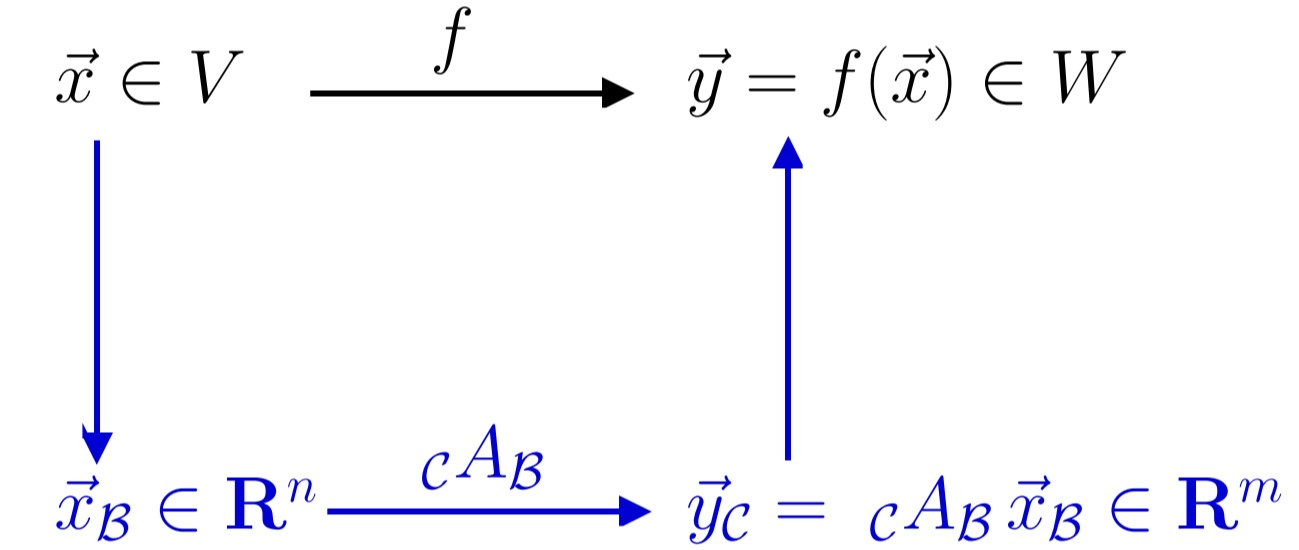
\includegraphics[scale=0.17]{abbildungsmatrix}
\end{center}

\ssect{Kern, Bild und Dimension}

Sei $f: V \rightarrow W$ eine lineare Abbildung von $V$ nach $W$.
Dann heisst die Menge $\ker(f) = \{ \vec{x} \in V \mid f(\vec{x}) = \vec{0} \in W \}$ der \textbf{Kern von $f$}.
Die Menge $\im(f) = \{ f(\vec{x}) \in W \mid \vec{x} \in V \}$ heisst das \textbf{Bild von $f$}.

\textbf{Satz:} Es gilt:
\begin{itemize}
    \item $\ker(f) = f^{-1}(\{ \vec{0} \})$, das Urbild von $\{ \vec{0} \}$.
    $\ker(f)$ ist ein Unterraum von $V$.
    \item $\im(f) = f(V)$, der Bildraum von $V$.
    $\im(f)$ ist ein Unterraum von $W$.
\end{itemize}

Es gilt:
\vspace{-0.8em}
\begin{align*}
    rg(A) &= \text{ \# der führenden Einsen in der Matrix $A$ auf ZSF} \\
    &= \text{ Maximale \# der l.u.\ Spaltenvektoren von $A$} \\
    &= \dim(\im(f))
\end{align*}
\vspace{-1.8em}

\textbf{Satz:} Seien $V$ und $W$ Vektorräume.
Sei $f: V \rightarrow W$ eine lineare Abbildung.
Dann ist:
\[\dim(V) = \dim(\ker(f)) + \dim(\im(f))\]

\sssect{Rezept zur Bestimmung von $\ker(f)$ und $\im(f)$}
\begin{enumerate}
    \item Wir bestimmen die Abbildungsmatrix $A$.
    \item Wir betrachten das homogene lineare LGS $A \vec{x} = \vec{0}$ und wenden das Gauss-Verfahren an.
    \item $\ker(f)$ und $\im(f)$ können wie folgt abgelesen werden:
    \begin{itemize}
        \item $\ker(f)$ ist die Lösungsmenge von $A \vec{x} = \vec{0}$ und $\dim(\ker(f)) = $ Anzahl der freien Variablen.
        \item $\dim(\im(f)) = $ Anzahl der führenden Variablen.
        Die führenden Einsen zeigen eine mögliche Auswahl von linear unabhängigen Spaltenvektoren der Abbildungsmatrix $A$.
        Diese Spaltenvektoren bilden eine Basis von $\im(f)$.
    \end{itemize}
\end{enumerate}

\ssect{Eigenschaften}

Es seien $f: V \rightarrow W$ und $g: V \rightarrow W$ lineare Abbildungen mit den Darstellungsmatrizen $A, B$.
Es gilt:
\begin{itemize}
    \item Die Abbildung $f + g$ ist linear und wird durch $A + B$ dargestellt.
    \item Für $k \in \R$ ist die Abbildung $k \ f$ linear und wird durch $k \ A$ dargestellt.
\end{itemize}

Es seien $f: V \rightarrow W$ und $g: W \rightarrow Z$ lineare Abbildungen mit den Darstellungsmatrizen $A \in \R^{r \times n}$ und $B \in \R^{m \times r}$.
Dann ist die Komposition $g \comp f$ linear und wird durch $BA$ dargestellt.

\textbf{Satz:} Sei $\dim(V) = \dim(W) = n$ und $f: V \rightarrow W$ eine lineare Abbildung mit der $n \times n$ Darstellungsmatrix $A$.
\begin{itemize}
    \item Die folgenden Äquivalenzen gelten:
    \begin{alignat*}{2}
        f \text{ ist bijektiv} &\Leftrightarrow \ker(f) = \{ \vec{0}_V \} &&\Leftrightarrow \im(f) = W \\ &\Leftrightarrow rg(A) = n &&\Leftrightarrow A \text{ ist invertierbar} \\
        &\Leftrightarrow \det(A) \neq 0
    \end{alignat*}
    \item Ist die lineare Abbildung $f$ bijektiv, dann ist die Umkehrabbildung $f^{-1}: W \rightarrow V$ linear und bijektiv.
    Die Darstellungsmatrix von $f^{-1}$ ist $A^{-1}$, die Inverse zu $A$.
\end{itemize}

\ssect{Basiswechsel}

Seien $\B = (\vec{b}_1, \dots, \vec{b}_n)$ und $\C = (\vec{c}_1, \dots, \vec{c}_n)$ zwei Basen des Vektorraumes $V$.
Dann nennt man die $n \times n$ Matrix ${_\C}T{_\B}$, deren Spaltenvektoren die Koordinatenvektoren der Basisvektoren $\vec{b}_k \in \B$ bzgl.\ Basis $\C$ sind, die \textbf{Basistransformationsmatrix $\B$ auf $\C$}.
Es gilt also:
\[{_\C}T{_\B} = \leftidx{_\C}{\left( (\vec{b}_1)_\C \ \dots \ (\vec{b}_n)_\C \right)}{_\B} \]
Man kann sich $\B$ als \emph{alte} Basis und $\C$ als \emph{neue} Basis vorstellen.
Dann sind die Spalten von ${_\C}T{_\B}$ die alten Basisvektoren im neuen Gewand.

\textbf{Satz:} Die Basistransformationsmatrix ${_\C}T{_\B}$ von $\B$ auf $\C$ ist eindeutig bestimmt und invertierbar mit $({_\C}T{_\B})^{-1} = {_\B}T{_\C}$

Die \textbf{Basistransformationsmatrix} ${_\C}T{_\B}$ ergibt sich mit dem Gauss-Jordan-Verfahren
für zwei beliebige Basen:
\[\left( \vec{c}_1 \ \vec{c}_2 \mid \vec{b}_1 \ \vec{b}_2 \right) \Leftrightarrow \left( I_2 \mid {_\C}T{_\B} \right)\]

Wenn die alte Basis die Standardbasis ist, dann ist die Basistransformationsmatrix gleich der Inverse der Matrix, die durch die Basisvektoren der neuen Basis gebildet wird:
\[{_\B}T{_\S} = \leftidx{_\B}{\left( \vec{b}_1 \ \vec{b}_2 \ \vec{b}_3 \right)}{_\S^{-1}}\]
Ist die neue Basis die Standardbasis, dann ist die Basistransformationsmatrix gleich der Matrix, die durch die Basisvektoren der alten Basis gebildet wird:
\[{_\S}T{_\B} = \leftidx{_\S}{\left( \vec{b}_1 \ \vec{b}_2 \ \vec{b}_3 \right)}{_\B}\]

\textbf{Satz:} Gegeben sei ein $n$-dimensionaler Vektorraum $V$ mit zwei Basen $\B$ und $\C$ sowie eine lineare Abbildung $f: V \rightarrow V$.
Dann besteht zwischen den Abbildungsmatrizen ${_\B}A{_\B}$ und ${_\C}A{_\C}$ folgender Zusammenhang:
\[{_\C}A{_\C} = {_\C}T{_\B} \cdot {_\B}A{_\B} \cdot {_\B}T{_\C} = {_\C}T{_\B} \cdot {_\B}A{_\B} \cdot {_\C}T{_\B^{-1}}\]

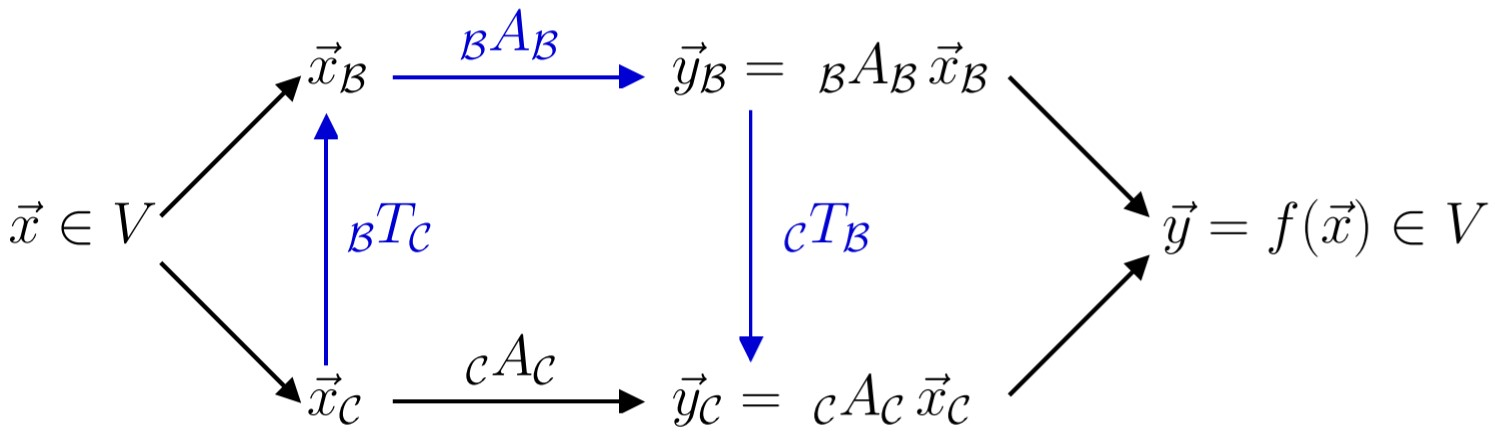
\includegraphics[scale=0.22]{basiswechsel}

\ssect{Geometrische Transformationen}

\sssect{Orthogonale Projektion}

\textbf{Orthogonalprojektion auf die $x$-Achse:}
\[\vec{x} \mapsto f(\vec{x}) = \left(
\begin{array}{cc}
    1 & 0 \\ 0 & 0
\end{array}
\right) \vec{x} = \left(
\begin{array}{c}
    x \\ 0
\end{array}
\right)\]

\textbf{Orthogonalprojektion auf die $y$-Achse:}
\[\vec{x} \mapsto f(\vec{x}) = \left(
\begin{array}{cc}
    0 & 0 \\ 0 & 1
\end{array}
\right) \vec{x} = \left(
\begin{array}{c}
    0 \\ y
\end{array}
\right)\]

\hrulefill

\begin{multicols}{2}
    \begin{itemize}
        \item Gerade $g: ax + by = 0$
        \item Mit $a^2 + b^2 = 1$
    \end{itemize}
    \[\left(
    \begin{array}{cc}
        1-a^2 & -ab \\ -ab & 1-b^2
    \end{array}
    \right)\]
\end{multicols}

\hrulefill

\begin{multicols}{2}
    \raggedright
    \begin{itemize}
        \item Gerade $g: 2x - y = 0$\\
        \item Normiert $g: \frac{2}{\sqrt{5}} x - \frac{1}{\sqrt{5}} y = 0$
    \end{itemize}
    \[\frac{1}{5} \cdot \left(
    \begin{array}{cc}
        1 & 2 \\ 2 & 4
    \end{array}
    \right)\]
\end{multicols}

\hrulefill

\textbf{Orthogonale Projektion auf die Ebene:}
\begin{itemize}
    \item $E: ax + by + cz = 0$
    \item $a^2 + b^2 + c^2 = 1$
\end{itemize}
\[P = \left(
\begin{array}{ccc}
    1-a^2 & -ab   & -ac   \\
    -ab   & 1-b^2 & -bc   \\
    -ac   & -bc   & 1-c^2
\end{array}
\right)\]
$P = E - \vec{n} \cdot \vec{n}^T$

\sssect{Spiegelung}

\textbf{Spiegelung an der $y$-Achse:}
\[\vec{x} \mapsto f_{S_y}(\vec{x}) = \left(
\begin{array}{cc}
    -1 & 0 \\ 0 & 1
\end{array}
\right) \vec{x} = \left(
\begin{array}{c}
    -x \\ y
\end{array}
\right)\]

\textbf{Spiegelung an der $x$-Achse:}
\[\vec{x} \mapsto f_{S_x}(\vec{x}) = \left(
\begin{array}{cc}
    1 & 0 \\ 0 & -1
\end{array}
\right) \vec{x} = \left(
\begin{array}{c}
    x \\ -y
\end{array}
\right)\]

\textbf{Spiegelung am Nullpunkt:}
\[\vec{x} \mapsto f_{S_N}(\vec{x}) = \left(
\begin{array}{cc}
    -1 & 0 \\ 0 & -1
\end{array}
\right) \vec{x} = \left(
\begin{array}{c}
    -x \\ -y
\end{array}
\right)\]

\hrulefill

\begin{multicols}{2}
    \begin{itemize}
        \item Gerade $g: ax + by = 0$
        \item Mit $a^2 + b^2 = 1$
    \end{itemize}
    \[\left(
    \begin{array}{cc}
        1 - 2a^2 & -2ab \\ -2ab & 1 - 2b^2
    \end{array}
    \right)\]
\end{multicols}

\hrulefill

\begin{multicols}{2}
    \raggedright
    \begin{itemize}
        \item Gerade $g: x + 7y = 0$
        \item Normiert $g: \frac{1}{\sqrt{50}}x + \frac{7}{\sqrt{50}}y = 0$
    \end{itemize}
    \[\frac{1}{50} \cdot \left(
    \begin{array}{cc}
        48 & -14 \\ -14 & -48
    \end{array}
    \right)\]
\end{multicols}

\hrulefill

\textbf{Spiegelung an der Ebene:}
\begin{itemize}
    \item $E: ax + by + cz = 0$
    \item $a^2 + b^2 + c^2 = 1$
\end{itemize}
\[S = \left(
\begin{array}{ccc}
    1-2a^2 & -2ab   & -2ac   \\
    -2ab   & 1-2b^2 & -2bc   \\
    -2ac   & -2bc   & 1-2c^2
\end{array}
\right)\]
$S = E - 2 \vec{n} \cdot \vec{n}^T$

\sssect{Streckung}

\textbf{Streckung längst der $x$-Achse um den Faktor $k$:}
\[\vec{x} \mapsto f_x(\vec{x}) = \left(
\begin{array}{cc}
    k & 0 \\
    0 & 1
\end{array}
\right) \vec{x} = \left(
\begin{array}{c}
    kx \\ y
\end{array}
\right)\]

\textbf{Streckung längst der $y$-Achse um den Faktor $k$:}
\[\vec{x} \mapsto f_y(\vec{x}) = \left(
\begin{array}{cc}
    1 & 0 \\
    0 & k
\end{array}
\right) \vec{x} \left(
\begin{array}{c}
    x \\ ky
\end{array}
\right)\]

\textbf{Zentrische Streckung vom Nullpunkt aus mit Faktor $k$:}
\[\vec{x} \mapsto f_{zs}(\vec{x}) = \left(
\begin{array}{cc}
    k & 0 \\
    0 & k
\end{array}
\right) \vec{x} = \left(
\begin{array}{c}
    kx \\ ky
\end{array}
\right)\]

\begin{center}
    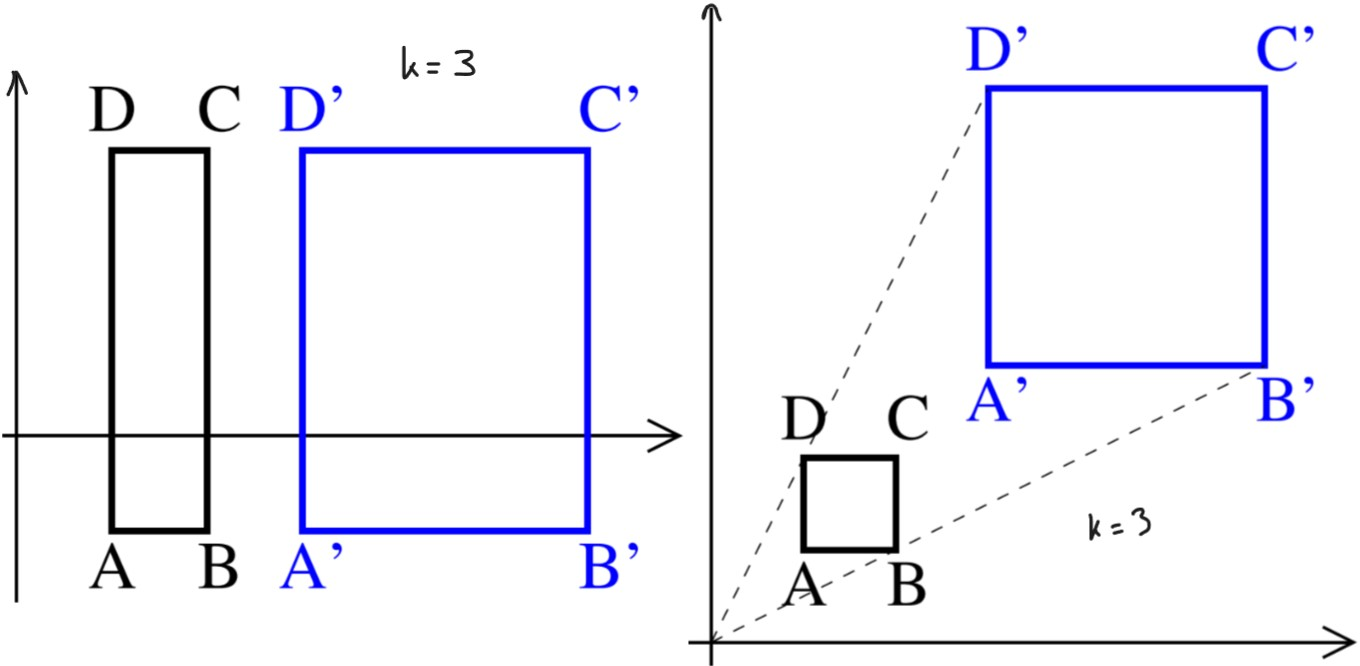
\includegraphics[scale=0.17]{streckung}
\end{center}

Faktor $\lambda$: $\left(
\begin{array}{ccc}
    \lambda & 0       & 0       \\
    0       & \lambda & 0       \\
    0       & 0       & \lambda
\end{array}
\right)$

\sssect{Scherung}

\textbf{Scherung längst der $x$-Achse mit Faktor $k$:}
\[\vec{x} \mapsto f(\vec{x}) = \left(
\begin{array}{cc}
    1 & k \\ 0 & 1
\end{array}
\right) \left(
\begin{array}{c}
    x \\ y
\end{array}
\right) = \left(
\begin{array}{c}
    x + ky \\ y
\end{array}
\right)\]

\textbf{Scherung längst der $y$-Achse mit Faktor $y$:}
\[\vec{x} \mapsto f(\vec{x}) = \left(
\begin{array}{cc}
    1 & 0 \\ k & 1
\end{array}
\right) \left(
\begin{array}{c}
    x \\ y
\end{array}
\right) = \left(
\begin{array}{c}
    x \\ kx + y
\end{array}
\right)\]

\sssect{Drehung}

\begin{multicols}{2}
    \begin{itemize}
        \item Um den Ursprung
        \item Um den Winkel $\varphi$
    \end{itemize}
    \[\left(
    \begin{array}{cc}
        \cos(\varphi) & -\sin(\varphi) \\
        \sin(\varphi) & \cos(\varphi)
    \end{array}
    \right)\]
\end{multicols}

\textbf{Drehung um den Winkel $\varphi$}

$x$-Achse: $\left(
\begin{array}{ccc}
    1 & 0             & 0              \\
    0 & \cos(\varphi) & -\sin(\varphi) \\
    0 & \sin(\varphi) & \cos(\varphi)
\end{array}
\right)$

$y$-Achse: $\left(
\begin{array}{ccc}
    \cos(\varphi)  & 0 & \sin(\varphi) \\
    0              & 1 & 0             \\
    -\sin(\varphi) & 0 & \cos(\varphi)
\end{array}
\right)$

$z$-Achse: $\left(
\begin{array}{ccc}
    \cos(\varphi) & -\sin(\varphi) & 0 \\
    \sin(\varphi) & \cos(\varphi)  & 0 \\
    0             & 0              & 1
\end{array}
\right)$